
\label{cap_conclusoes}

\indent

Neste trabalho, propomos a seguinte pergunta: fórmulas com menos cláusulas produzem respostas mais rápido? Como esforço para tentar responder esta pergunta, revisamos técnicas para reduzir o número de cláusulas geradas por uma fórmula proposicional, como as propostas por Boy de la Tour \cite{de1992optimality}, Nonnengart et al. \cite{nonnengart2001computing} e Jackson et al. \cite{jackson2004clause}, que são baseadas em renomeamento \cite{plaisted1986structure}. Após estudar estas técnicas, desenvolvemos também um algoritmo (Algoritmo \ref{knapsack}) baseado em programação dinâmica \cite{bellman2015applied} para obter renomeamentos que geram poucas cláusulas. Propomos ainda experimentos para: verificar uma propriedade de optimalidade restrita deste algoritmo; comparar este algoritmo com o de Boy de la Tour; e tentar responder a pergunta levantada inicialmente. Dos resultados experimentais obtidos, apresentados no Capítulo \ref{cap_resultados}, tiramos as seguintes conclusões principais:
\begin{enumerate}
	\item O esforço de tentar reduzir o tamanho de uma fórmula ao convertê-la para uma forma normal compensa na grande maioria das vezes;
	\item A representação de fórmulas através de DAGs é altamente recomendável para algoritmos de minimização baseados em renomeamento;
	\item É bastante provável que o algoritmo que propomos produza renomeamentos ótimos para árvores lineares. Propomos, como trabalho futuro, provar esta afirmação analiticamente;
	\item Diferentes algoritmos de renomeamento levam vantagem em diferentes famílias de fórmulas. Em particular, para as famílias \emph{SYJ206} e \emph{SYJ212} \cite{raths07jar}, o algoritmo que propomos gera muito menos cláusulas que o de Boy de la Tour;
	\item Por fim,...... (em construção)
\end{enumerate}

Um ponto ainda não explorado do algoritmo proposto é sua capacidade de obter bons renomeamentos com um dado limite fixo para o número de subfórmulas que podem ser escolhidas. Observamos que esta propriedade pode ser bastante útil, dado que as complexidades dos algoritmos de busca para SAT e VAL crescem justamente com o número de símbolos proposicionais de uma fórmula \cite{davis1960computing,davis1962machine,biere2009conflict}. Ao limitar o número de subfórmulas que podem ser escolhidas para renomeamento, deixamos de reduzir completamente o número de cláusulas, mas também impedimos que o número de símbolos proposicionais da transformação resultante cresça demais. Como trabalho futuro, propomos encontrar uma maneira de determinar um ponto limite ótimo para o número de subfórmulas que podem ser escolhidas para renomeamento. Esta ideia está ilustrada no gráfico da Figura \ref{limitando}. Uma vantagem adicional que pode surgir ao explorar este ponto é o fato de que um dos fatores lineares da complexidade do algoritmo vem justamente do número máximo de subfórmulas que podem ser escolhidas. No limite em que este número tende a zero, a complexidade do algoritmo tende a ficar quadrática, como a complexidade do algoritmo de Boy de la Tour. Portanto, o trabalho futuro agora proposto tem potencial para reduzir os tempos de execução de ambas as etapas: pré-processamento e busca.

\begin{figure}
	\begin{center}
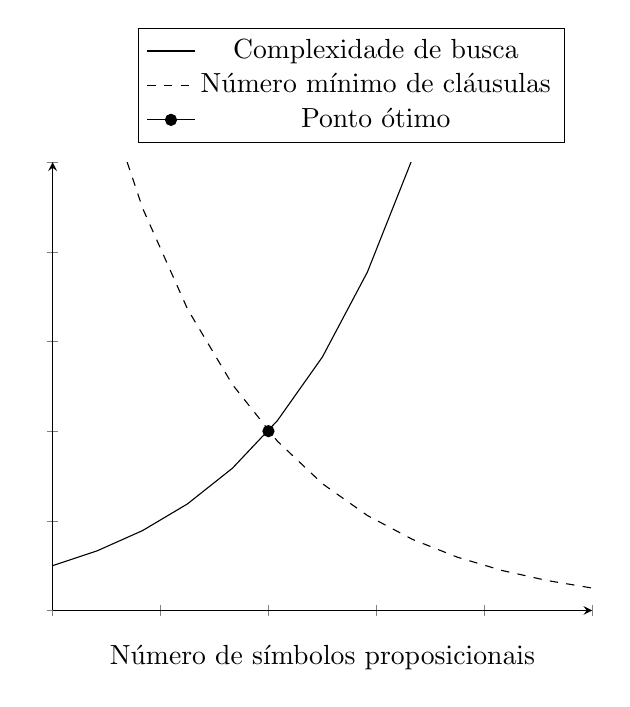
\begin{tikzpicture}
\begin{axis}[ymin=0,ymax=10,xmin=0,xlabel=Número de símbolos proposicionais,yticklabels={,,},xticklabels={,,},axis lines = left,legend entries={Complexidade de busca,Número mínimo de cláusulas,Ponto ótimo},legend style={at={(.95,1.3)}}]
\addplot[mark=none]{2^x};
\addplot[mark=none,dashed]{2^(4-x)};
\addplot[mark=*] coordinates {(2,4)};;
\end{axis}
\end{tikzpicture}
\end{center}
\label{limitando}
\caption{Ponto limite ótimo para o número de símbolos proposicionais.}
\end{figure}

Por último, observamos que o Algoritmo \ref{knapsack} se baseia principalmente na tomada de decisão da Linha 5. É provável que este critério possa ser apropriadamente substituído para resolver outros problemas, como minimização de outras formas normais, por exemplo. Como último trabalho futuro, deixamos a tarefa de investigar estas possíveis substituições.
